% !TEX program = xelatex
\documentclass[aspectratio=169]{beamer}

\usepackage{fontspec}
\usepackage{graphicx}
\usepackage{tikz}
\usepackage{amsmath}
\usepackage{booktabs}
\usepackage{tabularx}
\usepackage{array}
\usepackage{xcolor}
\usetikzlibrary{arrows.meta, positioning, shapes.geometric, fit}

\setsansfont{Noto Sans}
\setmainfont{Noto Sans}

\definecolor{DeepBlue}{HTML}{072A4A}
\definecolor{MidBlue}{HTML}{0D4D7C}
\definecolor{LightBlue}{HTML}{DDECF7}
\definecolor{Accent}{HTML}{3FA7D6}
\definecolor{SoftGray}{HTML}{F4F7FA}
\definecolor{DarkText}{HTML}{17324D}
\definecolor{WarnRed}{HTML}{C62828}
\definecolor{GoodGreen}{HTML}{2E7D32}

\usetheme{default}
\usecolortheme{default}
\setbeamertemplate{navigation symbols}{}
\setbeamertemplate{headline}{}
\setbeamercolor{background canvas}{bg=white}
\setbeamercolor{normal text}{fg=DarkText}
\setbeamercolor{frametitle}{fg=DeepBlue}
\setbeamerfont{frametitle}{size=\LARGE,series=\bfseries}
\setbeamerfont{title}{size=\Huge,series=\bfseries}
\setbeamerfont{subtitle}{size=\large}
\setbeamerfont{author}{size=\normalsize}
\setbeamerfont{date}{size=\small}

\setbeamertemplate{frametitle}{
  \vspace{0.35cm}
  \begin{beamercolorbox}[wd=\paperwidth,leftskip=0.65cm,rightskip=0.65cm]{frametitle}
    \insertframetitle
  \end{beamercolorbox}
  \vspace{-0.1cm}
  {\color{Accent}\rule{\paperwidth}{1.4pt}}
}

\setbeamertemplate{footline}{
  \leavevmode
  \begin{beamercolorbox}[wd=\paperwidth,ht=2.7ex,dp=1.0ex]{title in head/foot}
    \hspace{0.45cm}{\color{white}\scriptsize 11/05/2026}
    \hfill{\color{white}\scriptsize Few-shot detection trong video drone}
    \hfill{\color{white}\scriptsize \insertframenumber/\inserttotalframenumber}\hspace{0.45cm}
  \end{beamercolorbox}
}
\setbeamercolor{title in head/foot}{bg=DeepBlue}

\newcommand{\keyterm}[1]{\textbf{\color{MidBlue}#1}}
\newcommand{\tightitem}{\setlength\itemsep{0.42em}}
\newcommand{\imgcap}[1]{\par\vspace{0.05cm}{\scriptsize\color{DarkText}#1}\par}

\newenvironment{bluebox}[1]{
  \begin{beamercolorbox}[rounded=true,shadow=false,wd=\linewidth,sep=0.28cm]{block body}
  {\bfseries\color{DeepBlue}#1}\par\vspace{0.12cm}
}{
  \end{beamercolorbox}
}
\setbeamercolor{block body}{bg=SoftGray,fg=DarkText}

\title{PHÁT HIỆN MỤC TIÊU ÍT MẪU TỪ ẢNH DRONE}
\subtitle{Pipeline mới: YOLOE Visual Prompt + MobileCLIP2 + KCF}
\author{Nguyen Hung Quan -- 23521263 \quad | \quad Le Khac Thuan -- 23521550}
\institute{University of Information Technology\\Giảng viên: Huynh Tan Boi}
\date{11th May 2026}

\begin{document}

{
\setbeamertemplate{footline}{}
\begin{frame}[plain]
  \begin{tikzpicture}[remember picture,overlay]
    \fill[DeepBlue] (current page.south west) rectangle (current page.north east);
    \fill[MidBlue] ([xshift=-1.3cm,yshift=-0.9cm]current page.north east) circle (3.1cm);
    \fill[Accent,opacity=0.22] ([xshift=1.1cm,yshift=-1.0cm]current page.south west) circle (3.3cm);
  \end{tikzpicture}
  \vspace{0.2cm}
  {\color{LightBlue}\large University of Information Technology}\par
  \vspace{1.15cm}
  {\color{white}\bfseries\fontsize{34}{40}\selectfont PHÁT HIỆN MỤC TIÊU ÍT MẪU TỪ ẢNH DRONE}\par
  \vspace{0.45cm}
  {\color{LightBlue}\Large Few-shot object detection and tracking in drone video}\par
  \vfill
  {\color{white}\large Nguyen Hung Quan -- Le Khac Thuan}\par
  \vspace{0.15cm}
  {\color{LightBlue}\small 11th May 2026}
\end{frame}
}

\begin{frame}{Thành viên nhóm}
  \begin{columns}[T,onlytextwidth]
    \begin{column}{0.48\textwidth}
      \begin{bluebox}{Nguyen Hung Quan}
        \Large 23521263
      \end{bluebox}
    \end{column}
    \begin{column}{0.48\textwidth}
      \begin{bluebox}{Le Khac Thuan}
        \Large 23521550
      \end{bluebox}
    \end{column}
  \end{columns}
  \vspace{0.95cm}
  \begin{center}
    {\Large\bfseries\color{DeepBlue}Bài toán: từ 3 ảnh mẫu của một đối tượng, tìm đúng instance đó trong từng frame video drone.}
  \end{center}
\end{frame}

\begin{frame}{Nội dung}
  \begin{columns}[T,onlytextwidth]
    \begin{column}{0.48\textwidth}
      \begin{enumerate}
        \tightitem
        \item Bài toán và dữ liệu
        \item Preprocessing tạo visual prompt
        \item Pipeline mới trong repo
        \item YOLOE detector
      \end{enumerate}
    \end{column}
    \begin{column}{0.48\textwidth}
      \begin{enumerate}
        \setcounter{enumi}{4}
        \tightitem
        \item MobileCLIP2 matching và fusion
        \item KCF tracking
        \item Kết quả hiện tại
        \item Hạn chế và hướng phát triển
      \end{enumerate}
    \end{column}
  \end{columns}
\end{frame}

\begin{frame}{Bài toán}
  \small
  \begin{columns}[T,onlytextwidth]
    \begin{column}{0.54\textwidth}
      \begin{itemize}
        \tightitem
        \item Input mỗi sample gồm \keyterm{3 ảnh reference} và \keyterm{1 video drone}.
        \item Hệ thống cần định vị đúng đối tượng mục tiêu, không chỉ đúng class.
        \item Điều kiện khó: mục tiêu nhỏ, góc nhìn từ trên cao, nền phức tạp, scale thay đổi nhanh.
        \item Output là bounding box theo frame, score, JSON submission, report và biểu đồ thống kê.
      \end{itemize}
      \vspace{0.2cm}
      {\bfseries\color{DeepBlue}Yêu cầu thiết kế:} không train lại mô hình khi đổi đối tượng; chỉ đổi support images và video.
    \end{column}
    \begin{column}{0.42\textwidth}
      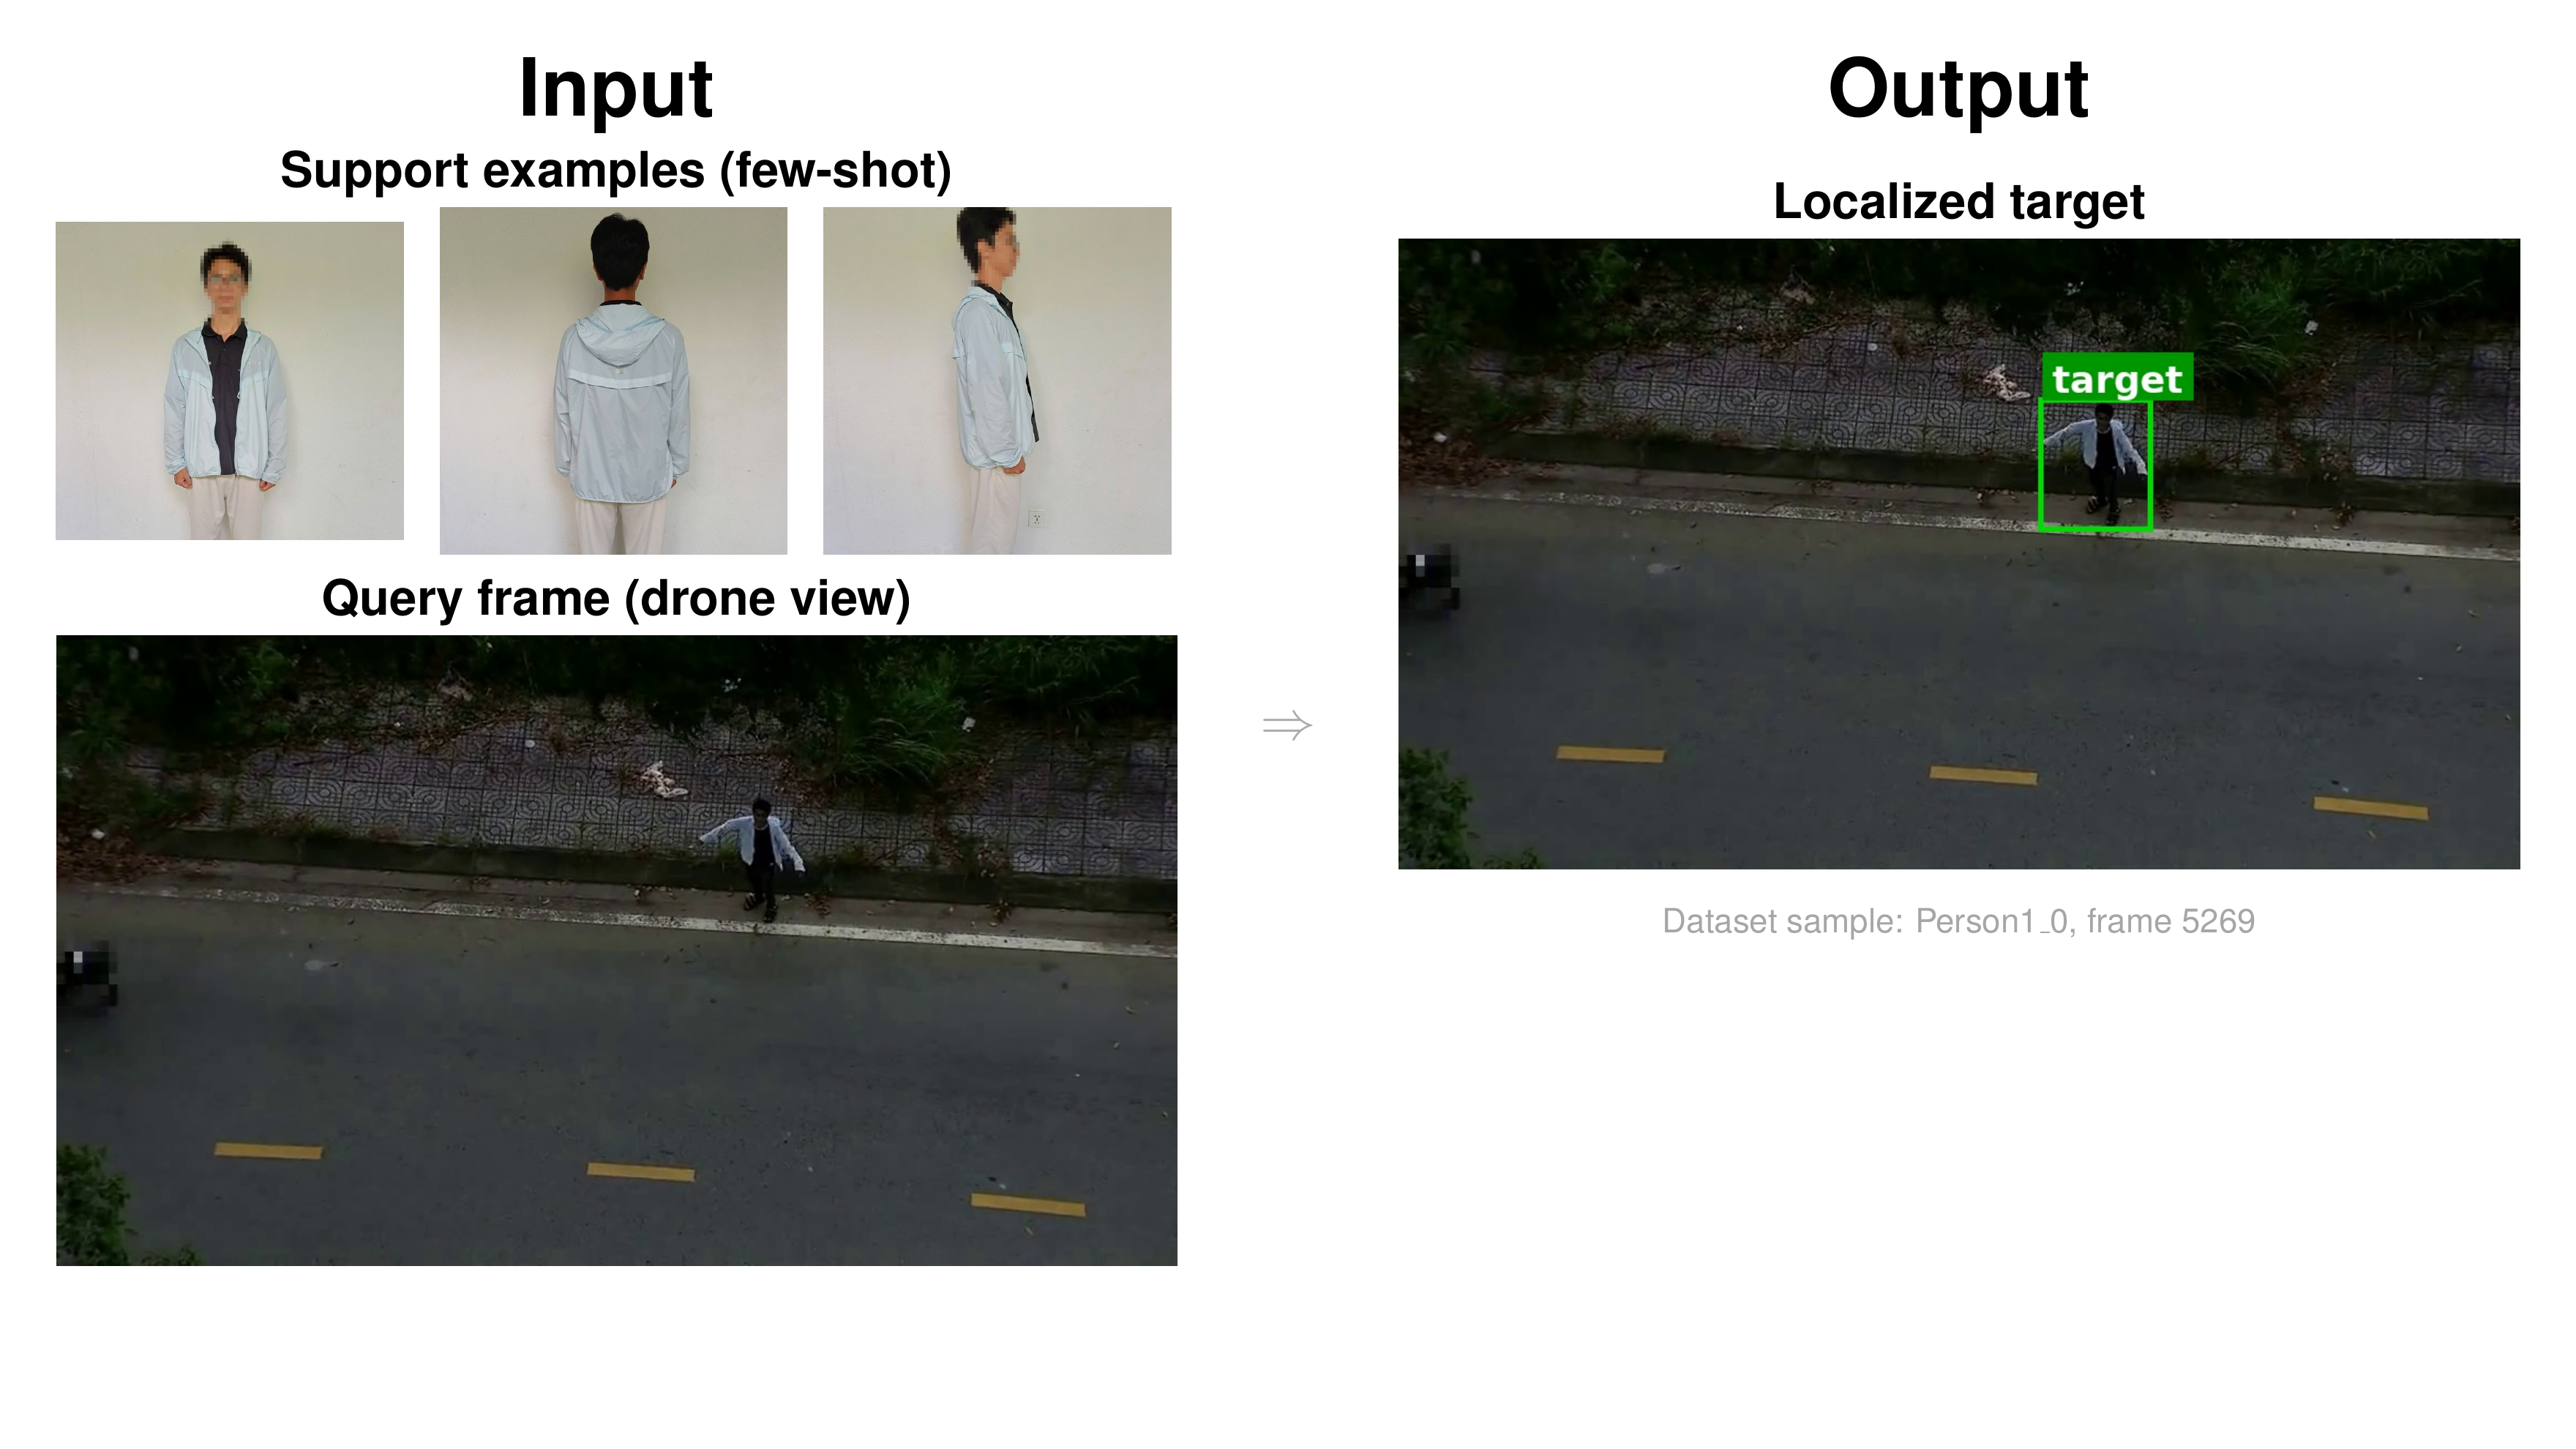
\includegraphics[width=\linewidth,height=0.30\textheight,keepaspectratio]{assets/fewshot_input_output_person1.png}
      \imgcap{Minh họa input few-shot và output bbox trong project.}
      \vspace{0.12cm}
      \begin{bluebox}{Input / Output}
        \scriptsize
        \begin{tabularx}{\linewidth}{>{\bfseries}lX}
          Input & 3 ảnh mẫu + video drone \\
          Output & BBox, score, JSON/report/plot \\
          Entry point & \texttt{./predict.sh} \\
        \end{tabularx}
      \end{bluebox}
    \end{column}
  \end{columns}
\end{frame}

\begin{frame}{Dữ liệu và Support Images}
  \footnotesize
  \begin{columns}[T,onlytextwidth]
    \begin{column}{0.50\textwidth}
      \begin{tabularx}{\linewidth}{>{\bfseries}lX}
        \toprule
        Phần & Vai trò \\
        \midrule
        Train & Có annotation; dùng để kiểm tra pipeline và tune threshold. \\
        Public test & Không có ground truth trong repo; dùng để xuất submission/report. \\
        Preprocess & Tạo VPE, reference crops và metadata cho từng sample. \\
        \bottomrule
      \end{tabularx}
      \vspace{0.18cm}
      \begin{bluebox}{Logic sử dụng dữ liệu}
        \scriptsize
        Pipeline không train lại theo class mới. Mỗi sample chỉ dùng 3 ảnh support để tạo visual prompt, sau đó tìm cùng instance trong video query.\par\vspace{0.08cm}
        Layout: \texttt{drone\_video.mp4} + \texttt{object\_images/*.jpg}.
      \end{bluebox}
    \end{column}
    \begin{column}{0.47\textwidth}
      {\bfseries\color{DeepBlue}Train support}\par\vspace{0.05cm}
      \begin{minipage}{0.31\linewidth}
        \centering
        \includegraphics[width=\linewidth,height=0.105\textheight,keepaspectratio]{data/train/samples/Backpack_0/object_images/img_1.jpg}
        {\tiny Backpack}
      \end{minipage}\hfill
      \begin{minipage}{0.31\linewidth}
        \centering
        \includegraphics[width=\linewidth,height=0.105\textheight,keepaspectratio]{data/train/samples/Person1_0/object_images/img_1.jpg}
        {\tiny Person}
      \end{minipage}\hfill
      \begin{minipage}{0.31\linewidth}
        \centering
        \includegraphics[width=\linewidth,height=0.105\textheight,keepaspectratio]{data/train/samples/WaterBottle_0/object_images/img_1.jpg}
        {\tiny Bottle}
      \end{minipage}

      \vspace{0.18cm}
      {\bfseries\color{DeepBlue}Public test support}\par\vspace{0.05cm}
      \begin{minipage}{0.31\linewidth}
        \centering
        \includegraphics[width=\linewidth,height=0.105\textheight,keepaspectratio]{data/public_test/samples/BlackBox_0/object_images/img_1.jpg}
        {\tiny BlackBox}
      \end{minipage}\hfill
      \begin{minipage}{0.31\linewidth}
        \centering
        \includegraphics[width=\linewidth,height=0.105\textheight,keepaspectratio]{data/public_test/samples/CardboardBox_0/object_images/img_1.jpg}
        {\tiny Cardboard}
      \end{minipage}\hfill
      \begin{minipage}{0.31\linewidth}
        \centering
        \includegraphics[width=\linewidth,height=0.105\textheight,keepaspectratio]{data/public_test/samples/LifeJacket_0/object_images/img_1.jpg}
        {\tiny LifeJacket}
      \end{minipage}
      \imgcap{Mỗi sample có 3 ảnh support; ở đây chọn một ảnh đại diện.}
    \end{column}
  \end{columns}
\end{frame}

\begin{frame}{Preprocessing}
  \centering
  \begin{tikzpicture}[
    node distance=0.42cm,
    pstep/.style={align=center, inner sep=0pt},
    lbl/.style={font=\scriptsize\bfseries, text=DeepBlue, align=center},
    arrow/.style={-{Latex[length=2.5mm]}, very thick, color=Accent}
  ]
    \node[pstep] (s1) {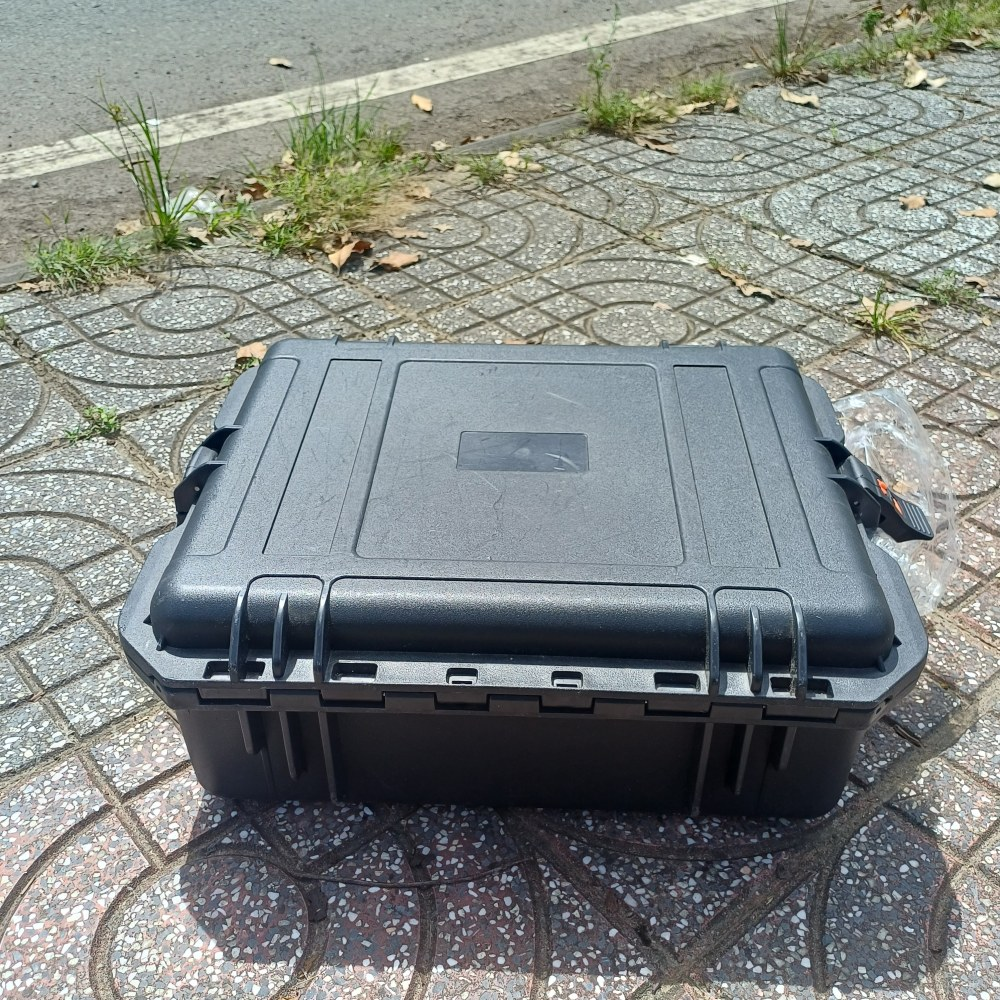
\includegraphics[width=2.65cm,height=1.45cm,keepaspectratio]{figures/preprocessing/support_blackbox0.jpg}};
    \node[lbl, below=0.06cm of s1] {1. Ảnh support};

    \node[pstep, right=of s1] (s2) {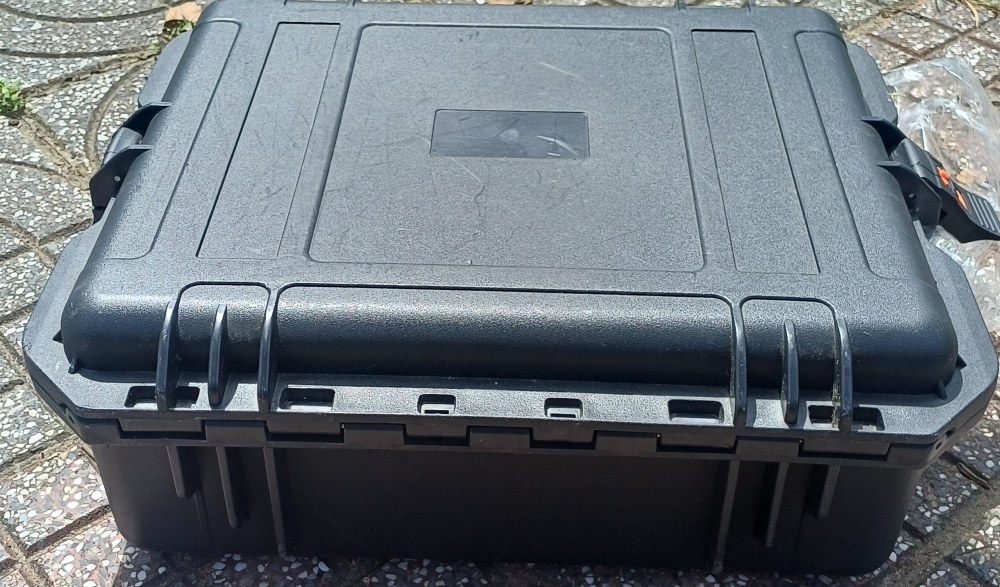
\includegraphics[width=2.65cm,height=1.45cm,keepaspectratio]{figures/preprocessing/reference_crop_blackbox0.jpg}};
    \node[lbl, below=0.06cm of s2] {2. Crop object};

    \node[pstep, right=of s2] (s3) {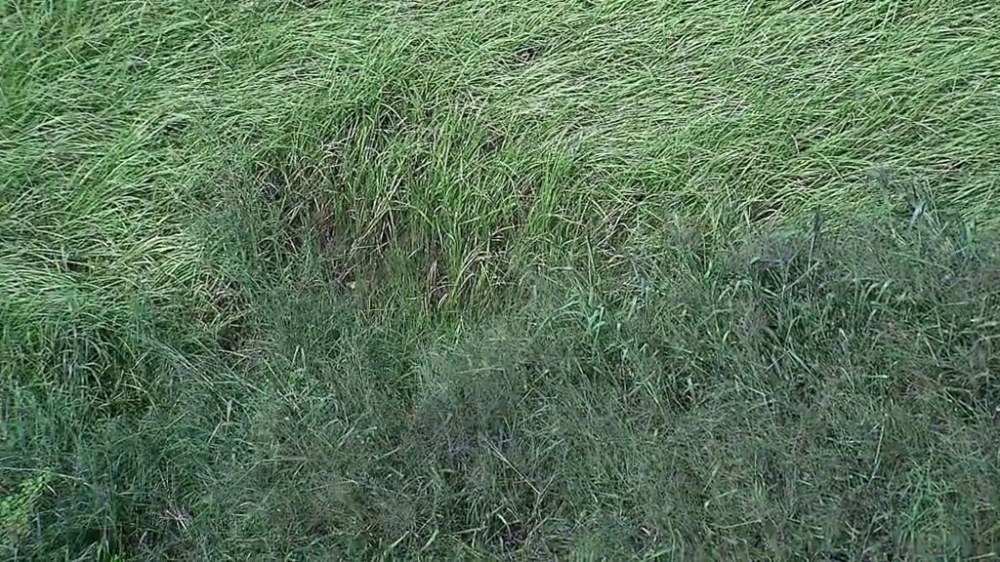
\includegraphics[width=2.65cm,height=1.45cm,keepaspectratio]{figures/preprocessing/query_background_blackbox0.jpg}};
    \node[lbl, below=0.06cm of s3] {3. Frame nền};

    \node[pstep, right=of s3] (s4) {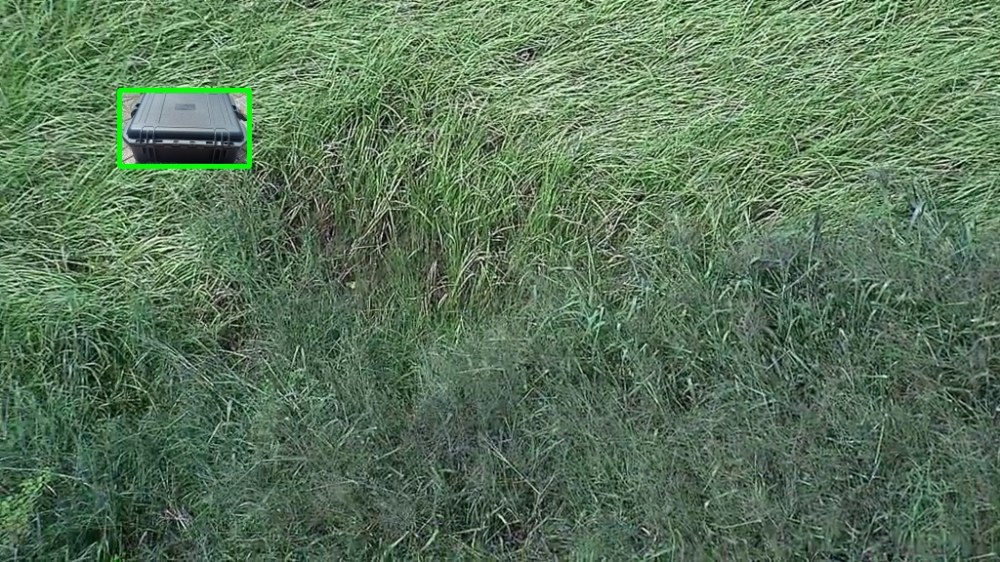
\includegraphics[width=2.65cm,height=1.45cm,keepaspectratio]{figures/preprocessing/augmented_prompt_blackbox0.jpg}};
    \node[lbl, below=0.06cm of s4] {4. Prompt tổng hợp + VPE};

    \draw[arrow] (s1) -- (s2);
    \draw[arrow] (s2) -- (s3);
    \draw[arrow] (s3) -- (s4);
  \end{tikzpicture}

  \vspace{0.28cm}
  \begin{columns}[T,onlytextwidth]
    \begin{column}{0.55\textwidth}
      \small
      \begin{enumerate}
        \setlength\itemsep{0.28em}
        \item Đọc 3 ảnh support từ \texttt{object\_images}.
        \item Dùng YOLOv8n detect và crop object từ từng ảnh support.
        \item Lấy frame nền từ video query để làm augmentation.
        \item Từ prompt tổng hợp, YOLOE sinh \keyterm{Visual Prompt Embedding}; lưu VPE, reference crops và metadata.
      \end{enumerate}
    \end{column}
    \begin{column}{0.41\textwidth}
      \begin{bluebox}{Config hiện tại}
        \scriptsize
        \begin{tabular}{ll}
          Reference crops & 3 / sample \\
          Augmented backgrounds & 4 / sample \\
          VPE image size & 640 \\
          Siamese checkpoint & Không dùng \\
          Seed & 42 \\
        \end{tabular}
      \end{bluebox}
    \end{column}
  \end{columns}
\end{frame}

\begin{frame}{Logic chọn Model}
  \footnotesize
  \begin{columns}[T,onlytextwidth]
    \begin{column}{0.49\textwidth}
      \begin{bluebox}{Bài toán không phù hợp với detector đóng class}
        \scriptsize
        Object public test đổi theo sample, mỗi sample chỉ có 3 ảnh mẫu.\par
        Vì vậy pipeline sinh candidate trước, rồi so khớp candidate với support để chọn instance đúng.
      \end{bluebox}
      \vspace{0.16cm}
      \begin{itemize}
        \tightitem
        \item \keyterm{YOLOE}: sinh bbox candidate theo visual prompt.
        \item \keyterm{MobileCLIP2}: lọc candidate bằng similarity với support.
        \item \keyterm{KCF}: khai thác liên tục thời gian giữa các frame.
      \end{itemize}
    \end{column}
    \begin{column}{0.47\textwidth}
      \begin{tabularx}{\linewidth}{>{\bfseries}lX}
        \toprule
        Khối & Lý do dùng \\
        \midrule
        Proposal & Không bỏ sót object nhỏ. \\
        Matching & Chọn đúng instance, không chỉ đúng class. \\
        Fusion & Kết hợp độ tin detector và độ giống support. \\
        Tracking & Giữ bbox ổn định giữa các frame. \\
        \bottomrule
      \end{tabularx}
    \end{column}
  \end{columns}
\end{frame}

\begin{frame}{Pipeline mới trong Project}
  \centering
  \begin{tikzpicture}[
    node distance=0.27cm,
    box/.style={draw=MidBlue, fill=LightBlue, rounded corners=2pt, very thick,
      align=center, minimum width=1.58cm, minimum height=0.80cm, font=\scriptsize\bfseries},
    outbox/.style={draw=DeepBlue, fill=DeepBlue, text=white, rounded corners=2pt, very thick,
      align=center, minimum width=1.55cm, minimum height=0.80cm, font=\scriptsize\bfseries},
    arrow/.style={-{Latex[length=2mm]}, very thick, color=MidBlue}
  ]
    \node[box] (input) {K-shot\\ảnh mẫu};
    \node[box, right=of input] (prep) {Preprocess\\VPE + crops};
    \node[box, right=of prep] (det) {YOLOE\\proposal};
    \node[box, right=of det] (clip) {MobileCLIP2\\matching};
    \node[box, right=of clip] (fusion) {Fusion\\det + clip};
    \node[box, right=of fusion] (trk) {KCF\\tracking};
    \node[outbox, right=of trk] (out) {BBox +\\score};

    \node[box, below=0.65cm of det, minimum width=2.35cm] (video) {Video drone\\query frame};

    \draw[arrow] (input) -- (prep);
    \draw[arrow] (prep) -- (det);
    \draw[arrow] (det) -- (clip);
    \draw[arrow] (clip) -- (fusion);
    \draw[arrow] (fusion) -- (trk);
    \draw[arrow] (trk) -- (out);
    \draw[arrow] (video) -- (det);
    \draw[arrow] (video) -- (clip);
    \draw[arrow] (video) -- (trk);
  \end{tikzpicture}

  \vspace{0.45cm}
  \begin{itemize}
    \tightitem
    \item \texttt{predict.sh} chạy theo thứ tự: preprocess support set \(\rightarrow\) inference từng video \(\rightarrow\) xuất JSON/report/plot.
    \item YOLOE ưu tiên recall, MobileCLIP2 ưu tiên đúng instance, fusion quyết định bbox cuối, KCF giữ tính liên tục theo thời gian.
    \item \textbf{Không còn Siamese trong main inference}; phần Siamese chỉ dùng để tham khảo/so sánh với hướng cũ.
  \end{itemize}
\end{frame}

\begin{frame}{Kiến trúc Module}
  \small
  \begin{tabularx}{\linewidth}{>{\bfseries}lX}
    \toprule
    Module & Vai trò trong pipeline mới \\
    \midrule
    \texttt{config.py} & Gom cấu hình inference, model path, data path; loại hard-code khỏi entry point. \\
    \texttt{detector.py} & \texttt{YOLOEDetector}: set visual prompt và sinh top-K proposals từ từng frame. \\
    \texttt{matcher.py} & \texttt{MobileCLIP2Matcher}: encode support/candidate crops và tính cosine similarity. \\
    \texttt{fusion.py} & Chuẩn hóa detector confidence, aggregate support score, gộp detector + CLIP + tracker bonus. \\
    \texttt{tracker.py} & Wrapper OpenCV KCF, init/update/reset qua một interface thống nhất. \\
    \texttt{inference.py} & \texttt{FewShotDetectionPipeline}: điều phối toàn bộ video, xuất JSON/report/plot. \\
    \bottomrule
  \end{tabularx}
  \vspace{0.22cm}
  {\small\bfseries\color{DeepBlue}Điểm khác pipeline cũ:}
  {\small Siamese không còn trong main inference; fusion hiện tại chỉ dùng detector score, CLIP score và tracker bonus.}
\end{frame}

\begin{frame}{YOLOE Detector}
  \begin{columns}[T,onlytextwidth]
    \begin{column}{0.56\textwidth}
      \begin{itemize}
        \tightitem
        \item Vai trò của YOLOE không phải chốt kết quả cuối, mà là tạo \keyterm{proposal} cho object được mô tả bằng support images.
        \item Preprocess đã biến 3 ảnh support thành \keyterm{initial VPE}; inference chỉ cần nạp VPE này cho từng sample.
        \item Mỗi frame được chạy với confidence rất thấp để không bỏ sót object nhỏ trong góc nhìn drone.
        \item Output giữ \texttt{top\_k=24} bbox/mask tốt nhất; các bbox này sẽ được MobileCLIP2 kiểm tra lại.
      \end{itemize}
    \end{column}
    \begin{column}{0.40\textwidth}
      \begin{bluebox}{Input / Output}
        \scriptsize
        Input: query frame + VPE của sample.\par
        Output: danh sách candidate gồm bbox \texttt{xyxy}, bbox \texttt{xywh}, confidence và mask nếu có.\par
        Ý nghĩa: tăng recall trước, xử lý false positive ở bước sau.
      \end{bluebox}
      \begin{bluebox}{Model / thông số}
        \scriptsize
        \begin{tabular}{ll}
          YOLOE & \texttt{yoloe-11l-seg.pt} \\
          Fallback & \texttt{yoloe-11s-seg.pt} \\
          Confidence & 0.001 \\
          Top-K proposals & 24 \\
          Retina masks & Bật \\
        \end{tabular}
      \end{bluebox}
    \end{column}
  \end{columns}
\end{frame}

\begin{frame}{MobileCLIP2 Matching}
  \begin{columns}[T,onlytextwidth]
    \begin{column}{0.53\textwidth}
      \begin{itemize}
        \tightitem
        \item YOLOE tạo candidate; MobileCLIP2 kiểm tra candidate nào thật sự giống 3 ảnh support.
        \item Support crops được encode một lần khi bắt đầu video và dùng lại cho mọi frame.
        \item Candidate bbox được crop, padding nhẹ, encode thành embedding rồi tính cosine similarity trung bình với support.
      \end{itemize}
    \end{column}
    \begin{column}{0.43\textwidth}
      \begin{bluebox}{Input / Output}
        \scriptsize
        Input: reference crops + candidate crops từ YOLOE.\par
        Output: similarity score cho từng candidate.\par
        Ý nghĩa: chuyển bài toán từ ``phát hiện class'' sang ``so khớp instance''.
      \end{bluebox}
      \begin{bluebox}{Config chính}
        \scriptsize
        \begin{tabular}{ll}
          Model & MobileCLIP2-S0 \\
          Encoder & \texttt{mobileclip2\_...\_fp16.pt} \\
          Aggregation & \texttt{mean} \\
        \end{tabular}
      \end{bluebox}
    \end{column}
  \end{columns}
\end{frame}

\begin{frame}{Score Fusion và Reference Gallery}
  \begin{columns}[T,onlytextwidth]
    \begin{column}{0.50\textwidth}
      \begin{itemize}
        \tightitem
        \item Detector score đo độ tin của proposal; CLIP score đo độ giống với support.
        \item Fusion normalize detector confidence theo frame rồi cộng trọng số với CLIP score.
        \item Candidate có fused score cao nhất và vượt threshold mới được ghi vào output.
        \item Crop có điểm rất cao được thêm vào reference gallery, giới hạn 20 crop để giảm drift.
      \end{itemize}
    \end{column}
    \begin{column}{0.46\textwidth}
      \begin{bluebox}{Công thức đang dùng}
        \scriptsize
        \[
          S = 0.30S_{det} + 0.35S_{clip} + S_{tracker}
        \]\vspace{-0.2cm}
        \par
        Nếu \(S \geq 0.52\), bbox được accept. Nếu không, frame đó không xuất bbox.
      \end{bluebox}
      \begin{bluebox}{Thông số chính}
        \scriptsize
        \begin{tabular}{ll}
          Fused threshold & 0.52 \\
          Weight detector & 0.30 \\
          Weight CLIP & 0.35 \\
          Tracker bonus & 0.04 \\
          Max reference samples & 20 \\
        \end{tabular}
      \end{bluebox}
    \end{column}
  \end{columns}
\end{frame}

\begin{frame}{KCF Tracking}
  \begin{columns}[T,onlytextwidth]
    \begin{column}{0.55\textwidth}
      \begin{itemize}
        \tightitem
        \item Video có tính liên tục: bbox frame hiện tại thường gần bbox frame trước.
        \item Khi một candidate được fusion accept, KCF được init bằng bbox đó để theo dõi các frame kế tiếp.
        \item Tracker giảm số lần chạy detector/matcher và làm bbox ổn định hơn khi object chưa đổi mạnh.
        \item Pipeline vẫn re-run detector định kỳ sau 10 frame hoặc khi tracker lỗi / bbox gần biên để tránh trôi mục tiêu.
      \end{itemize}
    \end{column}
    \begin{column}{0.41\textwidth}
      \begin{bluebox}{Input / Output}
        \scriptsize
        Input: frame hiện tại + bbox đã accept ở frame trước.\par
        Output: bbox dự đoán cho frame mới hoặc trạng thái fail.\par
        Ý nghĩa: thêm thông tin thời gian, nhưng không thay thế detector.
      \end{bluebox}
      \begin{bluebox}{Interface trong \texttt{tracker.py}}
        \scriptsize
        \begin{tabular}{ll}
          Backend ưu tiên & \texttt{cv2.TrackerKCF} \\
          Fallback & \texttt{cv2.legacy.TrackerKCF} \\
          API & \texttt{init}, \texttt{update}, \texttt{reset} \\
          Re-init interval & 10 frame \\
        \end{tabular}
      \end{bluebox}
    \end{column}
  \end{columns}
\end{frame}

\begin{frame}{Luồng xử lý một Frame}
  \small
  \begin{columns}[T,onlytextwidth]
    \begin{column}{0.48\textwidth}
      \begin{enumerate}
        \tightitem
        \item Quyết định dùng tracker hay chạy detector.
        \item YOLOE sinh danh sách candidate bbox/mask.
        \item Normalize detector confidence trong frame.
        \item Crop từng candidate và encode bằng MobileCLIP2.
      \end{enumerate}
    \end{column}
    \begin{column}{0.48\textwidth}
      \begin{enumerate}
        \setcounter{enumi}{4}
        \tightitem
        \item Tính similarity với support gallery.
        \item Fuse detector score + CLIP score + tracker bonus.
        \item Accept candidate nếu vượt threshold 0.52.
        \item Ghi bbox/score vào JSON và cập nhật report/plot.
      \end{enumerate}
    \end{column}
  \end{columns}
  \vspace{0.35cm}
  \begin{bluebox}{Output format}
    \scriptsize
    \texttt{video\_id} \(\rightarrow\) các đoạn \texttt{detections} \(\rightarrow\) danh sách \texttt{bboxes}: frame, x1, y1, x2, y2, score.
  \end{bluebox}
\end{frame}

\begin{frame}{Thiết lập Chạy hiện tại}
  \small
  \begin{columns}[T,onlytextwidth]
    \begin{column}{0.50\textwidth}
      \begin{bluebox}{Lệnh chính}
        \scriptsize
        \texttt{./predict.sh}\par\vspace{0.15cm}
        Script chạy 2 bước: preprocess public test vào \texttt{preprocessed\_data/public\_test}, sau đó gọi \texttt{python inference.py}.
      \end{bluebox}
      \vspace{0.15cm}
      \begin{bluebox}{Thư viện chính}
        \scriptsize
        \texttt{torch}, \texttt{torchvision}, \texttt{ultralytics}, \texttt{opencv-contrib-python}, \texttt{matplotlib}, local \texttt{ml-mobileclip}.
      \end{bluebox}
    \end{column}
    \begin{column}{0.46\textwidth}
      \begin{bluebox}{Environment variables}
        \scriptsize
        \begin{tabular}{ll}
          \texttt{YOLOE\_CONF} & 0.001 \\
          \texttt{TOP\_K} & 24 \\
          \texttt{FUSED\_THRESHOLD} & 0.52 \\
          \texttt{W\_DET} & 0.30 \\
          \texttt{W\_CLIP} & 0.35 \\
          \texttt{NUM\_BACKGROUNDS} & 4 \\
          \texttt{VPE\_IMGSZ} & 640 \\
        \end{tabular}
      \end{bluebox}
    \end{column}
  \end{columns}
\end{frame}

\begin{frame}{Kết quả Định tính}
  \centering
  \begin{tabular}{cc}
    \begin{minipage}{0.45\textwidth}
      \centering
      \includegraphics[width=\linewidth,height=0.25\textheight,keepaspectratio]{result/debug_demo_check/final_best_12s_zoom_contact.jpg}
      \imgcap{BlackBox: bbox bám mục tiêu trong frame query.}
    \end{minipage}
    &
    \begin{minipage}{0.45\textwidth}
      \centering
      \includegraphics[width=\linewidth,height=0.25\textheight,keepaspectratio]{result/debug_demo_check/blackbox_submission_contact.jpg}
      \imgcap{Output bbox và score trong submission/debug.}
    \end{minipage}
    \\
    \begin{minipage}{0.45\textwidth}
      \centering
      \includegraphics[width=\linewidth,height=0.25\textheight,keepaspectratio]{result/debug_demo_check/final_15s_zoom_contact.jpg}
      \imgcap{Zoom vùng mục tiêu để kiểm tra trực quan.}
    \end{minipage}
    &
    \begin{minipage}{0.45\textwidth}
      \centering
      \includegraphics[width=\linewidth,height=0.25\textheight,keepaspectratio]{result/debug_demo_check/blackbox_15s_contact.jpg}
      \imgcap{Trường hợp khó: mục tiêu nhỏ, nền rộng từ drone.}
    \end{minipage}
  \end{tabular}
\end{frame}

\begin{frame}{Thống kê Public Test}
  \begin{columns}[T,onlytextwidth]
    \begin{column}{0.54\textwidth}
      \includegraphics[width=\linewidth]{result/submission_stats.png}
      \imgcap{Detection rate trên 6 video public test trong output hiện tại.}
    \end{column}
    \begin{column}{0.43\textwidth}
      \scriptsize
      \begin{tabularx}{\linewidth}{Xrr}
        \toprule
        \bfseries Video & \bfseries Frames & \bfseries Det.\,rate \\
        \midrule
        BlackBox\_0 & 5{,}443 & 40.40\% \\
        BlackBox\_1 & 5{,}776 & 40.41\% \\
        CardboardBox\_0 & 5{,}285 & 1.38\% \\
        CardboardBox\_1 & 5{,}942 & 2.32\% \\
        LifeJacket\_0 & 8{,}309 & 44.59\% \\
        LifeJacket\_1 & 4{,}820 & 41.74\% \\
        \bottomrule
      \end{tabularx}
      \vspace{0.15cm}
      {\color{DeepBlue}\bfseries Nhận xét:} BlackBox và LifeJacket đạt khoảng 40--45\%; CardboardBox là class khó nhất.
    \end{column}
  \end{columns}
\end{frame}

\begin{frame}{Đánh giá Hiện tại}
  \begin{columns}[T,onlytextwidth]
    \begin{column}{0.48\textwidth}
      \begin{bluebox}{Full public test}
        \scriptsize
        \begin{tabular}{lr}
          Số video & 6 \\
          Tổng processed frames & 35{,}575 \\
          Mean detection rate & 28.47\% \\
          Mean fused score & 0.560 \\
          Mean Det / CLIP & 1.000 / 0.744 \\
          Best video & LifeJacket\_0 (44.59\%) \\
          Worst video & CardboardBox\_0 (1.38\%) \\
        \end{tabular}
      \end{bluebox}
      \vspace{0.12cm}
      \begin{bluebox}{Tracker counters trong report}
        \scriptsize
        \begin{tabular}{lr}
          Tracker init count & 0 \\
          Successful updates & 0 \\
          Tracker bbox returns & 0 \\
        \end{tabular}
      \end{bluebox}
    \end{column}
    \begin{column}{0.48\textwidth}
      \begin{itemize}
        \tightitem
        \item Public test không có ground truth trong repo, nên chưa thể tính IoU/mAP chính thức.
        \item Detection rate ở đây là tỷ lệ frame có bbox được xuất, không phải độ chính xác tuyệt đối.
        \item Score hiện tại phản ánh confidence sau fusion detector + MobileCLIP2.
        \item CardboardBox thấp do đối tượng ít đặc trưng, màu/texture dễ lẫn với nền.
      \end{itemize}
    \end{column}
  \end{columns}
\end{frame}

\begin{frame}{Phân tích Kết quả}
  \begin{columns}[T,onlytextwidth]
    \begin{column}{0.55\textwidth}
      \begin{itemize}
        \tightitem
        \item \keyterm{YOLOE} giúp tạo proposal theo visual prompt mà không cần train lại theo class mới.
        \item \keyterm{MobileCLIP2} lọc lại proposal theo similarity với support crops, phù hợp bài toán instance-level.
        \item \keyterm{CardboardBox} cho thấy giới hạn của few-shot matching khi object gần giống nền.
        \item \keyterm{KCF} đã có trong code nhưng chưa đóng góp vào report full run hiện tại; cần kiểm tra backend/init trong lần chạy tiếp theo.
      \end{itemize}
    \end{column}
    \begin{column}{0.42\textwidth}
      \includegraphics[width=\linewidth,height=0.32\textheight,keepaspectratio]{result/debug_demo_check/blackbox_15s_contact.jpg}
      \imgcap{Mục tiêu nhỏ trong frame drone làm matching và tracking khó ổn định.}
      \vspace{0.1cm}
      \begin{bluebox}{Kết luận ngắn}
        \scriptsize
        Pipeline mới đã rõ module và chạy end-to-end; bước tiếp theo là đánh giá bằng ground truth và cải thiện class khó.
      \end{bluebox}
    \end{column}
  \end{columns}
\end{frame}

\begin{frame}{Hạn chế}
  \small
  \begin{columns}[T,onlytextwidth]
    \begin{column}{0.55\textwidth}
      \begin{itemize}
        \tightitem
        \item Chưa có ground truth public test trong repo, nên detection rate chỉ là proxy coverage.
        \item Confidence YOLOE thấp và top-K lớn tăng recall nhưng có rủi ro false positives.
        \item MobileCLIP2 crop-level matching nhạy với crop sai, object nhỏ, blur và nền giống object.
        \item Reference gallery có thể giúp khi đúng, nhưng có nguy cơ drift nếu thêm crop sai.
        \item Tracker KCF cần được kiểm tra lại vì report hiện tại chưa ghi nhận tracker update.
      \end{itemize}
    \end{column}
    \begin{column}{0.41\textwidth}
      \begin{bluebox}{Class khó nhất}
        \scriptsize
        CardboardBox\_0: 1.38\% detection rate\par
        CardboardBox\_1: 2.32\% detection rate\par\vspace{0.1cm}
        Nguyên nhân chính: hình dạng và màu sắc dễ lẫn với mặt đất/cỏ trong góc nhìn drone.
      \end{bluebox}
      \vspace{0.18cm}
      \includegraphics[width=\linewidth,height=0.25\textheight,keepaspectratio]{result/submission_stats.png}
    \end{column}
  \end{columns}
\end{frame}

\begin{frame}{Kết luận \& Hướng phát triển}
  \begin{columns}[T,onlytextwidth]
    \begin{column}{0.49\textwidth}
      \begin{bluebox}{Kết luận}
        \footnotesize
        \begin{itemize}
          \tightitem
          \item Pipeline mới đã chuyển sang kiến trúc module hóa, dễ debug và mở rộng.
          \item Main inference hiện dùng YOLOE visual prompt + MobileCLIP2 matching + score fusion.
          \item Siamese không còn trong pipeline chính, tránh nhầm với phiên bản cũ.
        \end{itemize}
      \end{bluebox}
    \end{column}
    \begin{column}{0.49\textwidth}
      \begin{bluebox}{Hướng phát triển}
        \footnotesize
        \begin{itemize}
          \tightitem
          \item Bổ sung ground truth để đo IoU, precision, recall, mAP.
          \item Tune lại threshold/fusion bằng validation có nhãn.
          \item Cải thiện CardboardBox bằng hard negatives và multi-scale crops.
          \item Kiểm tra lại KCF backend/init hoặc thay bằng tracker mạnh hơn.
        \end{itemize}
      \end{bluebox}
    \end{column}
  \end{columns}
\end{frame}

{
\setbeamertemplate{footline}{}
\begin{frame}[plain]
  \begin{tikzpicture}[remember picture,overlay]
    \fill[DeepBlue] (current page.south west) rectangle (current page.north east);
    \fill[MidBlue] ([xshift=1.2cm,yshift=0.2cm]current page.south west) circle (3.4cm);
    \fill[Accent,opacity=0.25] ([xshift=-1.5cm,yshift=-1.0cm]current page.north east) circle (3.2cm);
  \end{tikzpicture}
  \centering
  \vspace{2.0cm}
  {\color{white}\bfseries\fontsize{42}{48}\selectfont THANKS FOR WATCHING!}\par
  \vspace{0.7cm}
  {\color{LightBlue}\Large Q \& A}
\end{frame}
}

\end{document}
